\item A container has a base of \( 50 \, \text{cm} \times 5 \, \text{cm} \) and height \( 50 \, \text{cm} \), as shown in the figure. It has two parallel electrically conducting walls each of area \( 50 \, \text{cm} \times 50 \, \text{cm} \). The remaining walls of the container are thin and non-conducting. The container is being filled with a liquid of dielectric constant \( 3 \) at a uniform rate of \( 250 \, \text{cm}^3 \, \text{s}^{-1} \). What is the value of the capacitance of the container after \( 10 \) seconds?\\[2mm] [Given: Permittivity of free space \( \varepsilon_0 = 9 \times 10^{-12} \, \text{C}^2 \text{N}^{-1} \text{m}^{-2} \), the effects of the non-conducting walls on the capacitance are negligible]
    \begin{center}
        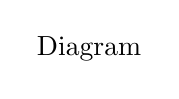
\begin{tikzpicture}
            \node {Diagram};
        \end{tikzpicture}
    \end{center}
        \begin{tasks}(2)
            \task \( 27 \, \text{pF} \)
            \task \( 63 \, \text{pF} \)\ans
            \task \( 81 \, \text{pF} \)
            \task \( 135 \, \text{pF} \)
        \end{tasks}